\paragraph{4. Do the lost relations result in New Observable Behaviors?}

        To answer this, we need to see whether the relations removed had an impact on possible $\stck{_{rf}}$ relations other than those with $e$. 
        We divide our argument into two parts, viz. the two types of relations removed:
        \begin{tasks}[style=enumerate](2)
            \task $\reln{k}{hb}{R_{uo}}$. 
            \task $\reln{R_{uo}}{hb}{k}$.
        \end{tasks}

        Figure~\ref{elim_read:case1} shows an exhaustive breakdown of sub-cases for case (1), varying based
        on the nature of event $k$.
        \begin{figure}[H]
            \centering
            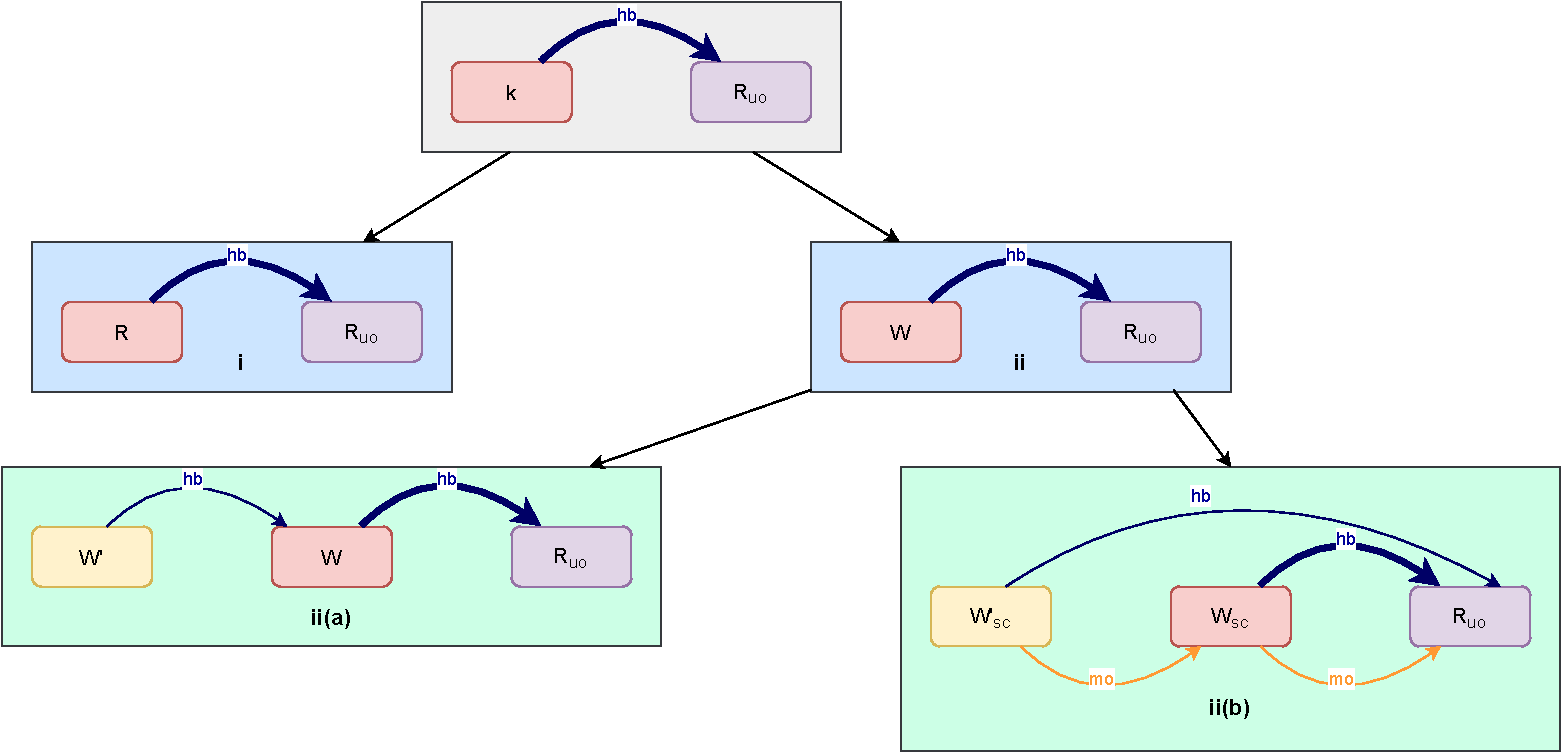
\includegraphics[scale=0.5]{5.Elimination/1.ValidEliminationCandidate/ReadElimProof/ProofParts/Part4_Case1.pdf}
            \caption{The impact of lost relation $\reln{k}{hb}{R_{uo}}$ on observable behaviors.}
            \label{elim_read:case1}
        \end{figure}

        Observations:
        \begin{itemize}
            \item For (i), when $k$ is a read, the pattern matches none of the Axioms.
            \item For (ii), when $k$ is a write, Axiom \ref{CoRe} (ii(a)) or Axiom \ref{SeqCsAt} (ii(b)) could restrict the read ($e$) from reading overlapping ranges of $W'$ with $W$.
        \end{itemize}

        Thus, for the case (1), we can conclude that the removed relations do not introduce any new observable behaviors.

        Figure~\ref{elim_read:case2} shows an exhaustive breakdown of sub-cases for case (2), varying based
        on the nature of event $k$.
        \begin{figure}[H]
            \centering
            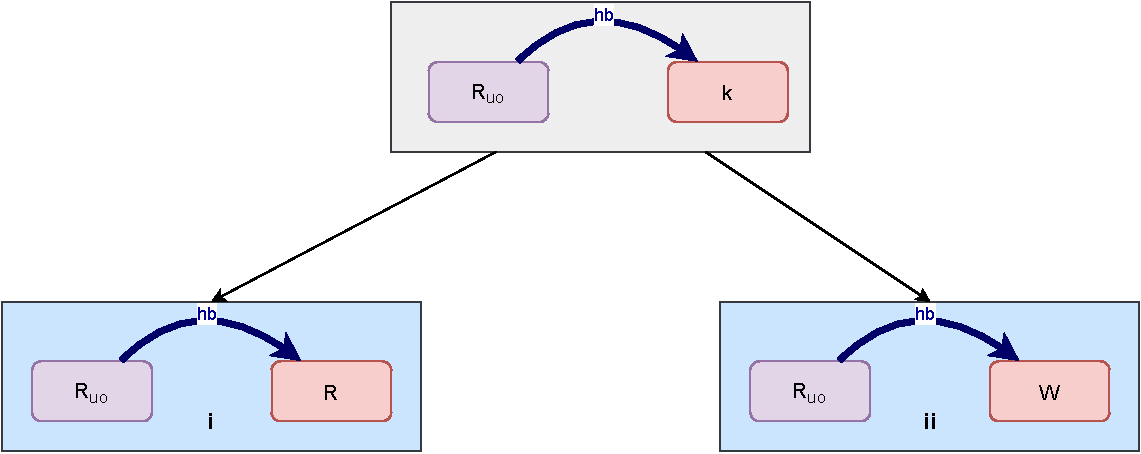
\includegraphics[scale=0.5]{5.Elimination/1.ValidEliminationCandidate/ReadElimProof/ProofParts/Part4_Case2.pdf}
            \caption{The impact of lost relation $\reln{R_{uo}}{hb}{k}$ on observable behaviors.}
            \label{elim_read:case2}
        \end{figure}

        Observations:
        \begin{itemize}
            \item Case (i) does not correspond to any pattern restricted by the Axioms of the model, thus having no impact on the observable behaviors. 
            \item For (ii), when $k$ is a write, Axiom \ref{CoRe} restricts the read $e$ from reading values of write $k$. 
        \end{itemize}

        Thus, for the case (2), we can conclude that the removed relations do not introduce any new observable behaviors.

        From the above observations, we can infer that the relations removed only have restriction on reads-from relations on the event $e$ we eliminate. 
        Thus, we can conclude that no new observable behaviors are introduced due to the removed $\stck{_{hb}}$ relations. 